\chapter{Schade aan het genoom en kanker}\label{ch:g11:cancer}

Onder de microscoop is een plakje gezonde darmbekleding een toonbeeld van
orde: \omterm{def:g10:cells-common-unit:cell}{cellen} in nette lagen, elk met een bescheiden kern, die onderin de
laag delen en bovenin sterven, keurig in de pas. Enkele millimeters
verderop, in datzelfde plakje, heeft een plek \omterm{def:g10:cells-common-unit:cell}{cellen} de gelederen
verbroken: dicht opeen, vreemd van vorm, met enorme donkere kernen, overal
delend en de weefsels eronder in dringend. Elke \omterm{def:g10:cells-common-unit:cell}{cel} van die plek stamt af
van één \omterm{def:g10:cells-common-unit:cell}{cel} die enkele jaren eerder een \omterm{def:g11:mutations:mutation}{mutatie} opliep die haar liet delen
waar dat niet had gemogen --- en daarna, in de loop van de jaren, nog
enkele. Dit hoofdstuk gaat over hoe de regelingen van de \omterm{def:g11:cell-cycle-mitosis:cycle}{celcyclus} falen,
wat ze beschadigt, en wat er vooraf en achteraf te doen valt.

\section{Delen wanneer het niet zou moeten}

\begin{definition}[Kanker]\label{def:g11:cancer:cancer}
\emph{Kanker}\index{kanker} is een populatie \omterm{def:g10:cells-common-unit:cell}{cellen} die zich delen zonder
de regelingen die de deling van normale \omterm{def:g10:cells-common-unit:cell}{cellen} begrenzen, en die de
omliggende weefsels binnendringen. Zij begint met één \omterm{def:g10:cells-common-unit:cell}{cel} waarvan het \omterm{def:g10:universal-dna:information}{DNA}
\omterm{def:g11:mutations:mutation}{mutaties} heeft opgehoopt in de \omterm{def:g10:universal-dna:gene}{genen} die de \omterm{def:g11:cell-cycle-mitosis:cycle}{celcyclus} besturen; de
nakomelingen van die \omterm{def:g10:cells-common-unit:cell}{cel} vormen een \emph{tumor}\index{tumor}. Een tumor
die op zijn plaats blijft, is \emph{goedaardig}; een tumor waarvan de
\omterm{def:g10:cells-common-unit:cell}{cellen} naburig weefsel binnendringen en via het bloed of de lymfe elders
nieuwe tumoren stichten (\emph{uitzaaiingen}), is \emph{kwaadaardig}.
\end{definition}

\begin{proposition}[Kanker is een ziekte van het genoom]\label{prop:g11:cancer:genome}
De \omterm{def:g10:cells-common-unit:cell}{cellen} van een \omterm{def:g11:cancer:cancer}{tumor} dragen \omterm{def:g11:mutations:mutation}{mutaties} die de andere \omterm{def:g10:cells-common-unit:cell}{cellen} van hun
eigenaar niet dragen: somatische \omterm{def:g11:mutations:mutation}{mutaties}, in één \omterm{def:g10:cells-common-unit:cell}{cel} ontstaan en door
haar nakomelingen geërfd. De \omterm{def:g11:cancer:cancer}{tumor} is een \emph{kloon}, en hij evolueert
--- \omterm{def:g10:cells-common-unit:cell}{cellen} die sneller delen of beter overleven nemen het over, en latere
\omterm{def:g11:mutations:mutation}{mutaties} voegen het vermogen toe om binnen te dringen en zich te
verspreiden.
\end{proposition}
\begin{proof}[Bewijsmateriaal]
Het \omterm{def:g10:universal-dna:information}{DNA} van tumorcellen naast dat van de normale \omterm{def:g10:cells-common-unit:cell}{cellen} van de patiënt
aflezen levert duizenden verschillen op, alle aanwezig in de \omterm{def:g11:cancer:cancer}{tumor} en
geen enkel in het gezonde weefsel; dezelfde handvol \omterm{def:g10:universal-dna:gene}{genen} blijkt in de
ene \omterm{def:g11:cancer:cancer}{tumor} na de andere gemuteerd. Elke tumorcel van een vrouw draagt
hetzelfde van haar twee \omterm{def:g10:universal-dna:information}{X-chromosomen} uitgeschakeld --- het handschrift
van afstamming uit één enkele \omterm{def:g10:cells-common-unit:cell}{cel}. En \omterm{def:g11:mutations:mutagen}{mutagenen} zijn \omterm{def:g11:cancer:carcinogen}{carcinogenen}: de
invloeden die het mutatietempo verhogen (\cref{ch:g11:mutations}) verhogen
het kankertempo, met tientallen jaren vertraging.
\end{proof}

\begin{omfigure}
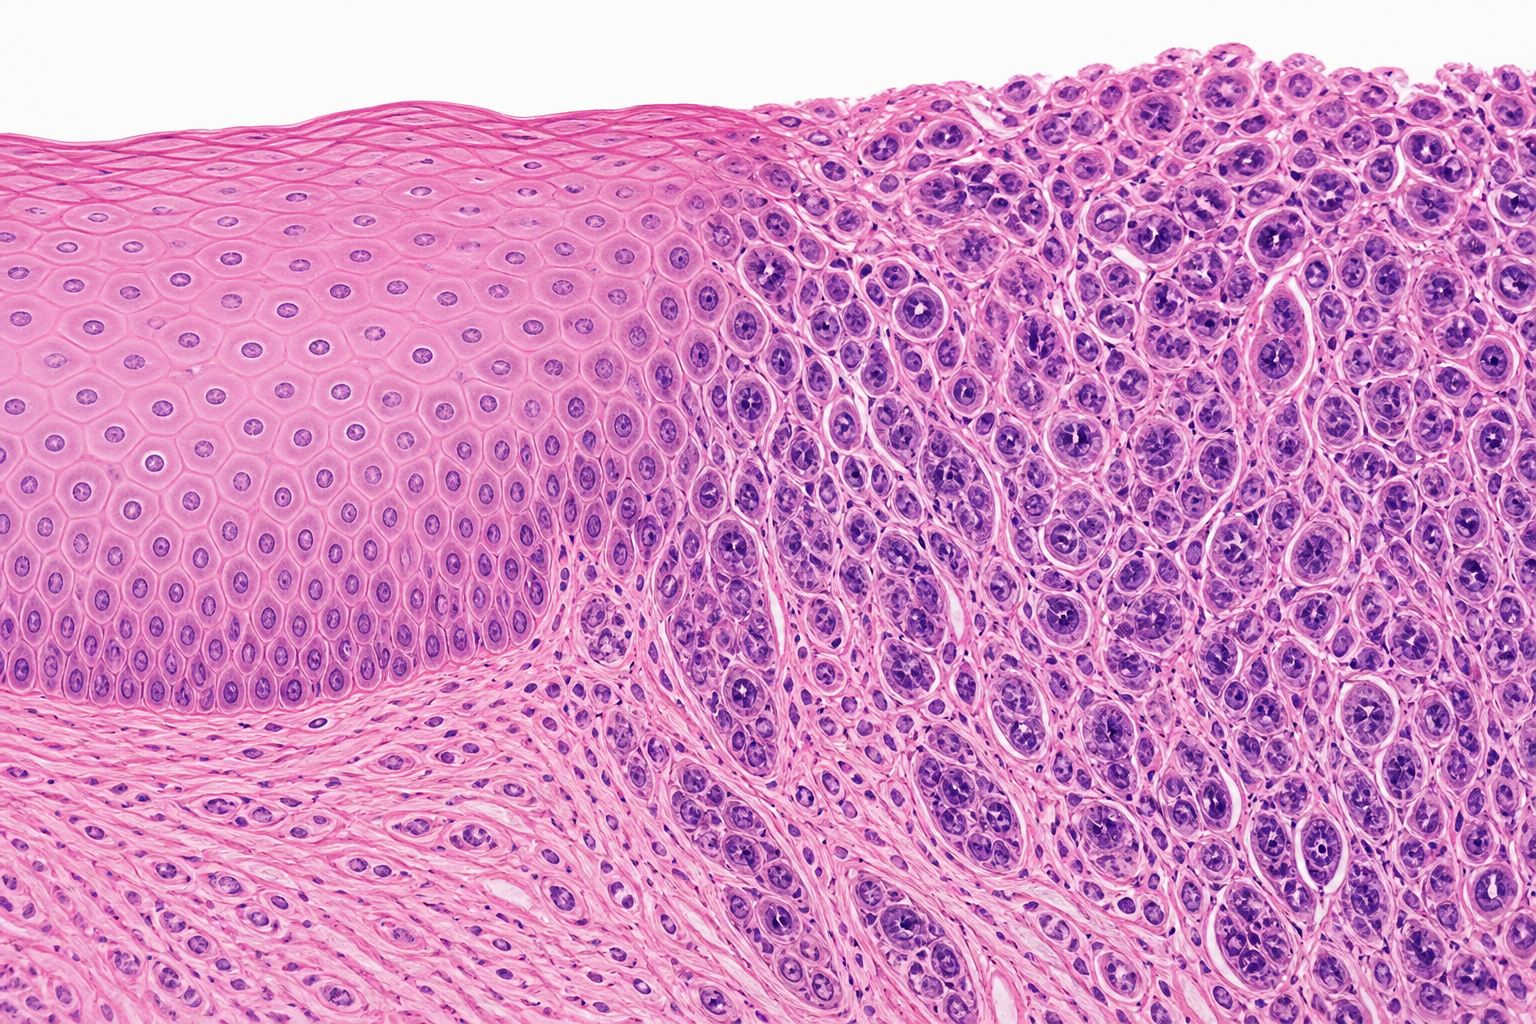
\includegraphics[width=0.62\linewidth]{images/book2/ai/g11-cancer-histology.png}

{\small Een gekleurde weefselcoupe: links nette \omterm{def:g10:cells-common-unit:cell}{cellen} in keurige lagen;
rechts een wanordelijke massa dicht opeengepakte \omterm{def:g10:cells-common-unit:cell}{cellen} met grote,
onregelmatige kernen die het weefsel in dringen. De grens tussen beide is
de grens van de \omterm{def:g11:cancer:cancer}{tumor}.}
\end{omfigure}

\section{Gaspedalen en remmen}

\begin{proposition}[Twee typen genen sturen de cyclus]\label{prop:g11:cancer:genes}
Het besluit van een \omterm{def:g10:cells-common-unit:cell}{cel} om zich te delen wordt genomen door \omterm{def:g10:chemistry-of-life:families}{eiwitten} die
als het gaspedaal en de remmen van een voertuig werken.
\begin{itemize}
  \item \emph{Proto-oncogenen}\index{proto-oncogen} coderen voor
        \omterm{def:g10:chemistry-of-life:families}{eiwitten} die de \omterm{def:g10:cells-common-unit:cell}{cel} de cyclus in duwen zodra er een groeisignaal
        binnenkomt --- receptoren voor groeisignalen, en de schakels die
        het signaal naar de kern brengen. Een \omterm{def:g11:mutations:mutation}{mutatie} die zo'n \omterm{def:g11:gene-expression:protein}{eiwit}
        blijvend werkzaam laat, maakt van het \omterm{def:g10:universal-dna:gene}{gen} een
        \emph{oncogen}: het gaspedaal zit vast ingetrapt. Eén gemuteerd
        \omterm{def:g10:universal-dna:gene}{allel} volstaat.
  \item \emph{Tumorsuppressorgenen}\index{tumorsuppressorgen} coderen
        voor \omterm{def:g10:chemistry-of-life:families}{eiwitten} die de cyclus stilleggen --- bij de controleposten
        vóór S en vóór de \omterm{def:g11:cell-cycle-mitosis:cycle}{mitose} --- wanneer het \omterm{def:g10:universal-dna:information}{DNA} beschadigd is, en
        die het herstel op gang brengen of, als de schade onherstelbaar
        is, de zelfvernietiging van de \omterm{def:g10:cells-common-unit:cell}{cel}. Een \omterm{def:g11:mutations:mutation}{mutatie} die zo'n \omterm{def:g11:gene-expression:protein}{eiwit}
        uitschakelt, neemt een rem weg; omdat de \omterm{def:g10:cells-common-unit:cell}{cel} twee \omterm{def:g10:universal-dna:gene}{allelen} heeft,
        moeten beide verloren gaan.
\end{itemize}
De bekendste suppressor, het \omterm{def:g11:gene-expression:protein}{eiwit} p53, is in de helft van alle
menselijke \omterm{def:g11:cancer:cancer}{kankers} uitgeschakeld.
\end{proposition}
\admitted

\begin{omfigure}
\begin{tikzpicture}[font=\small, >=Stealth,
  b/.style={draw, rounded corners, align=center, text width=2.8cm, minimum height=1.0cm}]
  \node[b, fill=omMeth!15] (sig) at (0,1.2) {groeisignaal\\ van andere cellen};
  \node[b, fill=omMeth!15] (onc) at (3.8,1.2) {eiwitten van\\ proto-oncogenen geven het door};
  \node[b, fill=omDef!15] (cyc) at (7.6,1.2) {de cel gaat\\ de cyclus in};
  \node[b, fill=omDef!15] (div) at (11.4,1.2) {deling};
  \draw[->, thick] (sig) -- (onc); \draw[->, thick] (onc) -- (cyc); \draw[->, thick] (cyc) -- (div);
  \node[b, fill=omThm!12] (dam) at (3.8,-1.4) {DNA-schade\\ opgemerkt};
  \node[b, fill=omThm!12, text width=3.1cm] (p53) at (7.6,-1.4) {tumorsuppressor-\\ eiwitten (p53\dots)};
  \node[b, fill=omThm!12, text width=3.4cm] (halt) at (11.4,-1.4) {leg de cyclus stil;\\ herstel, of zelfvernietiging};
  \draw[->, thick] (dam) -- (p53); \draw[->, thick] (p53) -- (halt);
  \draw[thick, omThm] (11.4,-0.85) -- (11.4,0.5);
  \draw[thick, omThm] (11.1,0.5) -- (11.7,0.5);
  \node[anchor=east, font=\scriptsize, omThm, align=right] at (11.0,-0.2) {rem};
  \node[anchor=west, font=\scriptsize, omMeth!60!black] at (0.2,2.05) {gaspedaal};
\end{tikzpicture}

{\small De regelingen van de deling. \omterm{def:g10:chemistry-of-life:families}{Eiwitten} van proto-oncogenen geven
groeisignalen door en duwen de \omterm{def:g10:cells-common-unit:cell}{cel} de cyclus in (het gaspedaal);
tumorsuppressoreiwitten leggen haar stil wanneer het \omterm{def:g10:universal-dna:information}{DNA} beschadigd is (de
rem). Een oncogen is een vastzittend gaspedaal; een verloren suppressor is
een weggenomen rem.}
\end{omfigure}

\begin{example}[Twee bekende genen]\label{ex:g11:cancer:genes}
Een receptor voor een groeisignaal zit in het membraan van veel \omterm{def:g10:cells-common-unit:cell}{cellen};
één substitutie in zijn \omterm{def:g10:universal-dna:gene}{gen} laat hem onafgebroken signaleren, zonder enig
signaal van buiten --- een oncogen dat in een derde van de dikkedarm- en
longkankers wordt gevonden. Het \omterm{def:g10:universal-dna:gene}{gen} van p53 wordt daarentegen op elke
denkbare manier uitgeschakeld: substituties die zijn vorm veranderen,
deleties, een voortijdige stop. Een \omterm{def:g10:cells-common-unit:cell}{cel} die p53 heeft verloren, houdt niet
in om haar \omterm{def:g10:universal-dna:information}{DNA} te herstellen voordat zij het kopieert, en hoopt dus
sneller nog meer \omterm{def:g11:mutations:mutation}{mutaties} op: die rem verliezen versnelt het hele proces.
\end{example}

\section{Verscheidene stappen, vele jaren}

\begin{proposition}[Kanker is een proces van vele stappen]\label{prop:g11:cancer:multistep}
Eén enkele \omterm{def:g11:mutations:mutation}{mutatie} maakt nog geen \omterm{def:g11:cancer:cancer}{kanker}. Een \omterm{def:g10:cells-common-unit:cell}{cel} moet er verscheidene
ophopen --- doorgaans één geactiveerd oncogen en twee of meer verloren
suppressoren --- en elke volgende \omterm{def:g11:mutations:mutation}{mutatie} vergroot, doordat zij de kloon
sneller laat groeien, het aantal \omterm{def:g10:cells-common-unit:cell}{cellen} waarin de volgende kan optreden.
Die reeks kost jaren tot tientallen jaren, en daarom stijgt het voorkomen
van de meeste \omterm{def:g11:cancer:cancer}{kankers} steil met de leeftijd, en daarom verschijnt de
werking van een \omterm{def:g11:cancer:carcinogen}{carcinogeen} twintig of dertig jaar na de blootstelling.
\end{proposition}
\begin{proof}[Bewijsmateriaal]
In de dikke darm zijn de stadia te zien: een kleine goedaardige poliep met
één suppressormutatie; een grotere poliep met daarbij een oncogen; een
binnendringende \omterm{def:g11:cancer:cancer}{tumor} waarin bovendien p53 verloren is --- een reeks van
zo'n vier tot zes \omterm{def:g11:mutations:mutation}{mutaties} over tien tot twintig jaar, waarbij elk stadium
in de \omterm{def:g10:cells-common-unit:cell}{cellen} van het volgende wordt teruggevonden. Het voorkomen van
\omterm{def:g11:cancer:cancer}{kanker} stijgt ruwweg met de vijfde macht van de leeftijd, de kromme die je
verwacht als er ongeveer vijf of zes onafhankelijke zeldzame
gebeurtenissen alle in één \omterm{def:g10:cells-common-unit:cell}{cel} moeten plaatsvinden. Mensen die één
gemuteerd \omterm{def:g10:universal-dna:gene}{allel} van een suppressorgen erven, krijgen de bijbehorende
\omterm{def:g11:cancer:cancer}{kanker} vroeger en vaker, omdat er in elke \omterm{def:g10:cells-common-unit:cell}{cel} al één stap is gezet.
\end{proof}

\begin{omfigure}
\begin{tikzpicture}[font=\small, >=Stealth]
  \tikzset{c/.style={circle, draw, inner sep=0, minimum size=0.28cm}}
  % stage 1: one normal cell mutates
  \foreach \x in {0,0.35,...,1.05} \foreach \y in {0,0.35,0.7} \node[c, fill=omDef!15] at (\x,\y) {};
  \node[c, fill=omProp!60] at (0.7,0.35) {};
  \node[anchor=north, align=center, text width=2.4cm] at (0.5,-0.4) {één cel krijgt\\ mutatie 1};
  \draw[->, thick] (1.5,0.35) -- (2.3,0.35) node[midway, above, font=\scriptsize] {jaren};
  % stage 2: clone
  \begin{scope}[xshift=2.7cm]
    \foreach \x in {0,0.35,...,1.4} \foreach \y in {0,0.35,0.7} \node[c, fill=omDef!15] at (\x,\y) {};
    \foreach \x in {0.35,0.7,1.05} \foreach \y in {0.35,0.7} \node[c, fill=omProp!60] at (\x,\y) {};
    \node[c, fill=omThm!70] at (0.7,0.35) {};
    \node[anchor=north, align=center, text width=2.6cm] at (0.7,-0.4) {haar kloon groeit;\\ één cel krijgt\\ mutatie 2};
  \end{scope}
  \draw[->, thick] (4.6,0.35) -- (5.4,0.35) node[midway, above, font=\scriptsize] {jaren};
  % stage 3: larger clone
  \begin{scope}[xshift=5.8cm]
    \foreach \x in {0,0.35,...,1.75} \foreach \y in {0,0.35,0.7,1.05} \node[c, fill=omProp!60] at (\x,\y) {};
    \foreach \x in {0.35,0.7,1.05,1.4} \foreach \y in {0.35,0.7} \node[c, fill=omThm!70] at (\x,\y) {};
    \node[c, fill=black!70] at (0.7,0.35) {};
    \node[anchor=north, align=center, text width=2.8cm] at (0.9,-0.4) {mutatie 3 in\\ de snelste kloon:\\ binnendringende kanker};
  \end{scope}
  \draw[->, thick] (8.0,0.35) -- (8.8,0.35) node[midway, above, font=\scriptsize] {jaren};
  \begin{scope}[xshift=9.2cm]
    \foreach \x in {0,0.35,...,2.1} \foreach \y in {0,0.35,0.7,1.05} \node[c, fill=omThm!70] at (\x,\y) {};
    \foreach \x in {0.35,0.7,...,1.75} \foreach \y in {0.35,0.7} \node[c, fill=black!70] at (\x,\y) {};
    \node[anchor=north, align=center, text width=2.6cm] at (1.05,-0.4) {tumor: een kloon\\ van klonen};
  \end{scope}
\end{tikzpicture}

{\small Klonale evolutie. Elke \omterm{def:g11:mutations:mutation}{mutatie} die de deling versnelt, vergroot de
kloon waarin de volgende \omterm{def:g11:mutations:mutation}{mutatie} kan optreden; na verscheidene van die
stappen, over jaren, heeft één lijn elke regeling verloren. De \omterm{def:g11:cancer:cancer}{tumor} is een
nest van klonen, de jongste binnen in de oudere.}
\end{omfigure}

\begin{omfigure}
\begin{tikzpicture}
\begin{axis}[
  width=0.86\linewidth, height=5.6cm,
  axis x line=bottom, axis y line=left,
  xmin=0, xmax=90, ymin=0, ymax=3200,
  xlabel={leeftijd (jaar)}, ylabel={nieuwe kankers per jaar per 100\,000},
  xlabel style={font=\small, at={(axis description cs:0.5,-0.12)}, anchor=north},
  ylabel style={font=\small},
  tick label style={font=\small}, xtick={0,20,40,60,80}, ytick={0,1000,2000,3000},
]
\addplot[thick, omThm, mark=*, mark size=1.4pt] coordinates
  {(5,20) (15,25) (25,45) (35,110) (45,300) (55,700) (65,1500) (75,2400) (85,3000)};
\end{axis}
\end{tikzpicture}

{\small Het aantal nieuwe \omterm{def:g11:cancer:cancer}{kankers} per jaar tegen de leeftijd (afgerond uit
landelijke registraties). De stijging is veel steiler dan evenredig: van
35 naar 70 verdubbelt de leeftijd en stijgt het voorkomen twintigvoudig,
het handschrift van verscheidene zeldzame gebeurtenissen die alle in één
\omterm{def:g10:cells-common-unit:cell}{cel} moeten plaatsvinden.}
\end{omfigure}

\section{Wat het genoom beschadigt}

\begin{definition}[Carcinogeen]\label{def:g11:cancer:carcinogen}
Een \emph{carcinogeen}\index{carcinogeen} is een invloed die het risico op
\omterm{def:g11:cancer:cancer}{kanker} verhoogt. De meeste zijn \omterm{def:g11:mutations:mutagen}{mutagenen}: het ultraviolet van het
zonlicht (huidkankers), de teer van tabaksrook (long, mond, blaas),
ioniserende straling, asbestvezels, alcohol, sommige schimmels. Andere
werken anders: bepaalde virussen dragen \omterm{def:g10:universal-dna:gene}{genen} die de remmen van de \omterm{def:g10:cells-common-unit:cell}{cel}
blokkeren --- humane papillomavirussen veroorzaken vrijwel alle
baarmoederhalskankers, hepatitisvirussen veel leverkankers --- en
langdurige ontsteking of hormonen die een weefsel aan het delen houden,
verhogen het aantal delingen waarin \omterm{def:g11:mutations:mutation}{mutaties} kunnen optreden.
\end{definition}

\begin{omfigure}
\begin{tikzpicture}
\begin{axis}[
  width=0.86\linewidth, height=5.4cm,
  axis x line=bottom, axis y line=left,
  xmin=0, xmax=45, ymin=0, ymax=30,
  xlabel={sigaretten per dag}, ylabel={relatief risico op longkanker},
  xlabel style={font=\small, at={(axis description cs:0.5,-0.12)}, anchor=north},
  ylabel style={font=\small},
  tick label style={font=\small}, xtick={0,10,20,30,40}, ytick={0,5,10,15,20,25,30},
]
\addplot[thick, omThm, mark=*, mark size=1.5pt] coordinates
  {(0,1) (5,6) (10,10) (15,14) (20,17) (25,20) (30,22) (40,25)};
\end{axis}
\end{tikzpicture}

{\small Het risico op longkanker ten opzichte van een niet-roker, tegen
het aantal sigaretten dat over tientallen jaren per dag is gerookt
(afgerond uit langlopend onderzoek). Het risico stijgt met de dosis, zoals
je van een \omterm{def:g11:mutations:mutagen}{mutageen} dat de longen bereikt verwacht.}
\end{omfigure}

\begin{example}[Tabak]\label{ex:g11:cancer:tobacco}
Rook draagt zo'n zeventig \omterm{def:g11:cancer:carcinogen}{carcinogenen}; benzopyreen, eenmaal door de
\omterm{def:g11:enzymes-and-phenotype:enzyme}{enzymen} van de \omterm{def:g10:cells-common-unit:cell}{cellen} zelf geactiveerd, hecht zich aan guanines en
veroorzaakt substituties op die plaatsen. Het p53-gen van een longtumor
van een roker draagt doorgaans precies zo'n substitutie, op een van de
weinige plaatsen waar benzopyreen zich het gemakkelijkst bindt --- het
\omterm{def:g11:mutations:mutagen}{mutageen} laat zijn handtekening in de volgorde achter. Longkanker was
vóór de sigaret een zeldzaamheid; roken veroorzaakt negen van de tien
gevallen, en stoppen halveert het risico binnen tien jaar, doordat de
\omterm{def:g10:cells-common-unit:cell}{cellen} die de eerste stappen droegen geleidelijk worden vervangen.
\end{example}

\begin{proposition}[Erfelijke aanleg]\label{prop:g11:cancer:inherited}
\omterm{def:g11:cancer:cancer}{Kanker} zelf wordt niet geërfd --- zij is een ziekte van somatische
\omterm{def:g11:mutations:mutation}{mutaties} --- maar een gemuteerd \omterm{def:g10:universal-dna:gene}{allel} van een suppressorgen wel. Wie één
niet werkend \omterm{def:g10:universal-dna:gene}{allel} van zo'n \omterm{def:g10:universal-dna:gene}{gen} erft, heeft in elke \omterm{def:g10:cells-common-unit:cell}{cel} van het lichaam
al één stap gezet; één enkele somatische \omterm{def:g11:mutations:mutation}{mutatie} van het andere \omterm{def:g10:universal-dna:gene}{allel}
maakt het verlies in elke \omterm{def:g10:cells-common-unit:cell}{cel} compleet, in plaats van de twee die anderen
nodig hebben. Het gevolg is een hoog risico op de bijbehorende \omterm{def:g11:cancer:cancer}{kankers}, en
dat op jongere leeftijd: zo'n 70\% van de vrouwen die een gemuteerd \omterm{def:g10:universal-dna:gene}{allel}
van een bepaald borstkankergen dragen, krijgt de ziekte, tegen 12\% in het
algemeen.
\end{proposition}
\admitted

\section{Voorkomen, opsporen, behandelen}

\begin{method}[Het risico verkleinen]\label{met:g11:cancer:prevention}
Omdat de meeste \omterm{def:g11:mutations:mutation}{mutaties} achter \omterm{def:g11:cancer:cancer}{kankers} uit aanwijsbare blootstellingen
komen, en omdat het proces jaren duurt, is \omterm{def:g11:cancer:cancer}{kanker} grotendeels te
voorkomen en op te sporen.
\begin{enumerate}
  \item \emph{Vermijd de \omterm{def:g11:mutations:mutagen}{mutagenen}}: geen tabak (een derde van alle
        sterfgevallen door \omterm{def:g11:cancer:cancer}{kanker}), weinig alcohol, bescherming tegen de
        zon, geen onnodige straling.
  \item \emph{Laat je inenten} tegen de virussen die \omterm{def:g11:cancer:cancer}{kanker} veroorzaken:
        het vaccin tegen het papillomavirus voorkomt vrijwel alle
        baarmoederhalskankers wanneer het vóór de blootstelling wordt
        gegeven.
  \item \emph{Screen}: spoor de \omterm{def:g11:cancer:cancer}{tumor} in het poliepstadium op ---
        uitstrijkjes van de baarmoederhals, darmonderzoek,
        borstonderzoek --- wanneer verwijderen eenvoudig is en geneest.
  \item \emph{Ken de familie}: een erfelijke aanleg vraagt om eerder en
        nauwgezetter toezicht.
\end{enumerate}
\end{method}

\begin{example}[Behandelingen en waar zij op mikken]\label{ex:g11:cancer:treatments}
Een operatie verwijdert een \omterm{def:g11:cancer:cancer}{tumor} die zich niet heeft verspreid.
Bestraling breekt het \omterm{def:g10:universal-dna:information}{DNA} van de \omterm{def:g10:cells-common-unit:cell}{cellen} in de bundel onherstelbaar en
doodt bij voorkeur delende \omterm{def:g10:cells-common-unit:cell}{cellen}. Chemotherapie gebruikt middelen die de
replicatie of de spoel blokkeren (\cref{ch:g11:cell-cycle-mitosis}):
tumorcellen, die onafgebroken delen, sterven sneller dan normale \omterm{def:g10:cells-common-unit:cell}{cellen}
--- maar ook de snel delende normale weefsels (beenmerg, darmbekleding,
haarwortels) lijden eronder, en daar komen de bijwerkingen vandaan.
Nieuwere behandelingen mikken op het bepaalde gemuteerde \omterm{def:g11:gene-expression:protein}{eiwit} van een
\omterm{def:g11:cancer:cancer}{tumor}, of laten het afweersysteem erop los.
\end{example}

\begin{remark}[Waarom wij allemaal het begin dragen]\label{rem:g11:cancer:everyone}
Elke volwassene draagt klonen \omterm{def:g10:cells-common-unit:cell}{cellen} met kankergerelateerde \omterm{def:g11:mutations:mutation}{mutaties} ---
in de huid, de darm, het bloed --- die nooit \omterm{def:g11:cancer:cancer}{kanker} worden: de overige
remmen houden stand, het afweersysteem ruimt de ergste op, en de persoon
sterft eerder aan iets anders. \omterm{def:g11:cancer:cancer}{Kanker} is de nu en dan optredende uitkomst
van een proces dat bij iedereen loopt; het doel van preventie is het
aantal gezette stappen, in welke \omterm{def:g10:cells-common-unit:cell}{cel} dan ook, onder het benodigde aantal
te houden.
\end{remark}

\section{Oefeningen}

\begin{exercise}[$\star$]\label{exo:g11:cancer:1}
Definieer \omterm{def:g11:cancer:cancer}{kanker}, \omterm{def:g11:cancer:cancer}{tumor} en uitzaaiing.
\end{exercise}

\begin{exercise}[$\star$]\label{exo:g11:cancer:2}
Wat is een proto-oncogen, en wat wordt het na een \omterm{def:g11:mutations:mutation}{mutatie}? Waarom
volstaat één gemuteerd \omterm{def:g10:universal-dna:gene}{allel}?
\end{exercise}

\begin{exercise}[$\star$]\label{exo:g11:cancer:3}
Wat doet een tumorsuppressoreiwit zoals p53? Waarom moeten beide \omterm{def:g10:universal-dna:gene}{allelen}
verloren gaan?
\end{exercise}

\begin{exercise}[$\star$]\label{exo:g11:cancer:4}
Noem vier \omterm{def:g11:cancer:carcinogen}{carcinogenen} en, voor twee ervan, de \omterm{def:g11:cancer:cancer}{kanker} die zij
veroorzaken.
\end{exercise}

\begin{exercise}[$\star$]\label{exo:g11:cancer:5}
Waarom wordt \omterm{def:g11:cancer:cancer}{kanker} een kloon genoemd?
\end{exercise}

\begin{exercise}[$\star\star$]\label{exo:g11:cancer:6}
Lees in de leeftijdsfiguur het voorkomen op 40 en op 80 af, en bereken de
factor. Vergelijk met de factor 2 in de leeftijd.
\end{exercise}

\begin{exercise}[$\star\star$]\label{exo:g11:cancer:7}
Geef uit de tabaksfiguur het relatieve risico bij 10 en bij 20 sigaretten
per dag. Als het levenslange risico van een niet-roker 1\% is, wat is dan
dat van iemand die er 20 per dag rookt?
\end{exercise}

\begin{exercise}[$\star\star$]\label{exo:g11:cancer:8}
Leg uit waarom een \omterm{def:g10:cells-common-unit:cell}{cel} die p53 heeft verloren, sneller nog meer \omterm{def:g11:mutations:mutation}{mutaties}
ophoopt dan een normale \omterm{def:g10:cells-common-unit:cell}{cel}.
\end{exercise}

\begin{exercise}[$\star\star$]\label{exo:g11:cancer:9}
Een vrouw erft één gemuteerd \omterm{def:g10:universal-dna:gene}{allel} van een suppressorgen voor
borstkanker. Leg in termen van "stappen" uit waarom haar risico hoog is
en haar \omterm{def:g11:cancer:cancer}{kankers} vroeg optreden; en waarom haar zussen één kans op twee op
hetzelfde lopen.
\end{exercise}

\begin{exercise}[$\star\star$]\label{exo:g11:cancer:10}
Waarom veroorzaken middelen voor chemotherapie haaruitval, misselijkheid
en een daling van het aantal witte bloedcellen?
\end{exercise}

\begin{exercise}[$\star\star$]\label{exo:g11:cancer:11}
Een roker die op zijn veertigste stopt, heeft op zijn zestigste de helft
van het longkankerrisico van iemand die is doorgegaan. Leg met het model
van de vele stappen uit waarom het risico daalt maar niet tot dat van een
niet-roker terugkeert.
\end{exercise}

\begin{exercise}[$\star\star\star$]\label{exo:g11:cancer:12}
Stel dat een \omterm{def:g11:cancer:cancer}{kanker} 3 bepaalde \omterm{def:g11:mutations:mutation}{mutaties} vergt, die elk met kans $10^{-7}$
per celdeling optreden. De stamcellen van een weefsel delen zich in een
leven $10^{12}$ keer. Schat het verwachte aantal \omterm{def:g10:cells-common-unit:cell}{cellen} dat de eerste
\omterm{def:g11:mutations:mutation}{mutatie} oploopt; leg met de klonale groei uit waarom het naïeve product
$10^{-21}$ voor alle drie veel te laag is.
\end{exercise}

\begin{exercise}[$\star\star\star$]\label{exo:g11:cancer:13}
Een papillomavirus draagt een \omterm{def:g10:universal-dna:gene}{gen} waarvan het \omterm{def:g11:gene-expression:protein}{eiwit} p53 bindt en
uitschakelt. Leg uit hoe het virus \omterm{def:g11:cancer:cancer}{kanker} veroorzaakt zonder enig
menselijk \omterm{def:g10:universal-dna:gene}{gen} te muteren, waarom het vaccin dat voorkomt, en waarom
inenten vóór de blootstelling van belang is.
\end{exercise}

\begin{exercise}[$\star\star\star$]\label{exo:g11:cancer:14}
Bij darmonderzoek op dikkedarmkanker wordt vanaf het vijftigste jaar om
de tien jaar gekeken en worden gevonden poliepen weggenomen. Leg met het
model van de vele stappen uit waarom dit \omterm{def:g11:cancer:cancer}{kanker} voorkomt in plaats van
haar alleen op te sporen, en waarom tien jaar een redelijke tussenpoos is.
\end{exercise}

\begin{exercise}[$\star\star\star$]\label{exo:g11:cancer:15}
"\omterm{def:g11:cancer:cancer}{Kanker} is een ziekte van de ouderdom, dus er valt niets aan te doen."
Bespreek dit in een alinea met de leeftijdskromme, de vertraging van
\omterm{def:g11:cancer:carcinogen}{carcinogenen}, het aandeel \omterm{def:g11:cancer:cancer}{kankers} dat aan bekende blootstellingen is toe
te schrijven, en de screening.
\end{exercise}

\section{Probleem: De handtekening in het gen}

\begin{problem}[{Weekendprobleem --- een longtumor afgelezen: de mutaties
geteld, de handtekening van de roker gelezen, de jaren berekend, en het
risico dat één sigaret draagt}]
\label{pb:g11:cancer:1}
Van een patiënt die 35 jaar lang 20 sigaretten per dag rookte, worden een
longtumor en gezond weefsel afgelezen. De \omterm{def:g11:cancer:cancer}{tumor} draagt $\num{5000}$
somatische substituties die in het gezonde weefsel niet voorkomen; 75\%
daarvan vervangt een G door een T, de verandering die benzopyreen
veroorzaakt. Daaronder: één in het p53-gen, die een voortijdige stop
schept, op één \omterm{def:g10:universal-dna:gene}{allel}; het andere \omterm{def:g10:universal-dna:gene}{allel} van p53 is verdwenen; en één in het
\omterm{def:g10:universal-dna:gene}{gen} van een receptor voor een groeisignaal, waardoor het \omterm{def:g11:gene-expression:protein}{eiwit} blijvend
werkzaam is.

\medskip
\noindent\textbf{Deel I --- De volgorde lezen.}
\begin{enumerate}
  \item Waarom heten de $\num{5000}$ substituties somatisch? Waar zouden
        zij te vinden zijn als zij tot de kiembaan behoorden?
  \item In de \omterm{def:g11:cancer:cancer}{tumor} van een niet-roker komen substituties van alle
        typen in ruwweg gelijke verhoudingen voor. Wat zegt de 75\%
        veranderingen van G naar T je?
  \item Deel de \omterm{def:g11:mutations:mutation}{mutatie} in p53 in (met de woorden van
        \cref{ch:g11:gene-expression}) en geef haar gevolg voor het
        \omterm{def:g11:gene-expression:protein}{eiwit}.
  \item Leg uit waarom beide \omterm{def:g10:universal-dna:gene}{allelen} van p53 verloren moesten gaan,
        terwijl één gemuteerd \omterm{def:g10:universal-dna:gene}{allel} van het receptorgen volstond.
  \item Welk van de twee \omterm{def:g10:universal-dna:gene}{genen} is een gaspedaal en welk een rem?
\end{enumerate}

\medskip
\noindent\textbf{Deel II --- De jaren.}
\begin{enumerate}[resume]
  \item De patiënt rookte ongeveer $20 \times 365 \times 35$ sigaretten.
        Bereken dat aantal.
  \item Hoeveel substituties zou een \omterm{def:g10:cells-common-unit:cell}{cel} na 35 jaar dragen als elke
        sigaret gemiddeld één blijvende substitutie in elk van de \omterm{def:g10:cells-common-unit:cell}{cellen}
        van de longbekleding oplevert? Vergelijk met de $\num{5000}$ die
        zijn gevonden.
  \item De \omterm{def:g11:mutations:mutation}{mutaties} van de \omterm{def:g11:cancer:cancer}{tumor} zitten niet alle in dezelfde \omterm{def:g10:cells-common-unit:cell}{cellen}: de
        \omterm{def:g11:mutations:mutation}{mutaties} in p53 en in de receptor zitten in elke tumorcel, de
        andere duizenden alleen in delen ervan. Wat zegt dat over wanneer
        de twee sleutelmutaties optraden?
  \item De \omterm{def:g11:cancer:cancer}{tumor} meet \qty{3}{cm} in doorsnee, ongeveer $10^{10}$ \omterm{def:g10:cells-common-unit:cell}{cellen},
        en tumorcellen verdubbelen om de 100 dagen. Hoeveel verdubbelingen
        vanaf één \omterm{def:g10:cells-common-unit:cell}{cel}, en hoeveel jaar op zijn minst?
  \item Combineer de vragen 8 en 9: ruwweg wanneer in die 35 jaar trad de
        laatste van de sleutelmutaties op?
\end{enumerate}

\medskip
\noindent\textbf{Deel III --- Het risico van één sigaret.}
\begin{enumerate}[resume]
  \item Volgens de tabaksfiguur was het relatieve risico van de patiënt
        ongeveer 17. Welk deel van de rokers zoals hij krijgt longkanker,
        als 1\% van de niet-rokers haar krijgt?
  \item Hoeveel van de \omterm{def:g11:cancer:cancer}{kankers} onder 100 zulke rokers zijn aan het roken
        toe te schrijven?
  \item Was hij op zijn veertigste gestopt (na 20 jaar), dan zou zijn
        risico ongeveer een derde van dat van de doorrokende zijn
        geweest. Leg met het model van de vele stappen en de vernieuwing
        van de longbekleding uit waarom het risico na het stoppen daalt.
  \item Waarom komt de \omterm{def:g11:cancer:cancer}{kanker} van een roker, als zij komt, meestal na
        dertig jaar en niet na vijf?
  \item Een leerling betoogt dat een sigaret onschadelijk is omdat zij
        "maar één \omterm{def:g11:mutations:mutation}{mutatie} per \omterm{def:g10:cells-common-unit:cell}{cel}" veroorzaakt. Antwoord met de
        rekensom van vraag 7 en het aantal \omterm{def:g10:cells-common-unit:cell}{cellen}.
\end{enumerate}

\medskip
\noindent\textbf{Deel IV --- Preventie en de bevolking.}
In een land van 60 miljoen inwoners rookt 25\% van de volwassenen;
longkanker doodt er $\num{30000}$ mensen per jaar, van wie 90\% roker is.
\begin{enumerate}[resume]
  \item Bereken het aantal sterfgevallen door longkanker per jaar onder
        rokers en onder niet-rokers, en het sterftecijfer per 100\,000 in
        elke groep (neem 45 miljoen volwassenen).
  \item Met welke factor ligt het cijfer bij rokers hoger? Vergelijk met
        het relatieve risico uit de figuur en becommentarieer dat.
  \item Wat zou het jaarlijkse aantal sterfgevallen door longkanker op
        lange termijn worden als het roken vandaag verdween? Waarom niet
        onmiddellijk?
  \item Screening met scans met een lage stralingsdosis vindt \omterm{def:g11:cancer:cancer}{tumoren}
        eerder en verlaagt de sterfte onder zware rokers met ongeveer
        20\%. Vergelijk, in vermeden sterfgevallen per jaar, elke roker
        screenen met stoppen met roken.
  \item Geef het resultaat: wat de handtekening van G naar T bewees over
        de oorsprong van de \omterm{def:g11:mutations:mutation}{mutaties} van de \omterm{def:g11:cancer:cancer}{tumor}, de drie genetische
        gebeurtenissen die de \omterm{def:g11:cancer:cancer}{kanker} maakten, en het ene besluit dat haar
        had voorkomen.
\end{enumerate}
\end{problem}
